\section{Collective Multi-agent Reasoning}
\label{sec:collective}

Building upon the single-agent foundation, where reasoning supports planning, search, and tool use within a unified perception–action loop, \textbf{multi-agent reasoning} extends these principles to collaborative settings. 
In a multi-agent system (MAS), multiple reasoning agents interact to jointly solve complex tasks. 
Rather than identical problem solvers, agents assume \emph{complementary roles}, such as \textit{Manager} for task decomposition, \textit{Worker} for execution, and \textit{Verifier} for evaluation, enabling specialization and division of cognitive labor. 
This role differentiation marks the first step toward collective intelligence, where reasoning is distributed and coordinated across multiple agents.

Beyond role assignment, the essence of multi-agent reasoning lies in how these agents \emph{collaborate, communicate, and co-evolve}. 
Collaboration schemas define how reasoning traces are exchanged, conflicts are resolved, and shared memory is maintained to achieve alignment. 
Through such interaction, reasoning transitions from an individual process into a distributed, iterative loop, in which agents refine each other’s outputs and collectively converge toward better solutions.

Compared with single-agent systems, multi-agent reasoning introduces new challenges that require rethinking reasoning at the system level:
\begin{itemize}
    \item \textbf{Role differentiation:} how to design static or adaptive roles that align with task structure and expertise distribution;
    \item \textbf{Collaboration and communication:} how agents exchange intermediate reasoning, negotiate consensus, and divide labor efficiently;
    \item \textbf{Collective memory and evolution:} how shared or distributed state supports long-term coordination and continual adaptation.
\end{itemize}

These challenges motivate the following structure of our analysis.
Section~\textbf{5.1} examines the \emph{role taxonomy} of multi-agent systems, from generic organizational roles to domain-specific specializations. 
Section~\textbf{5.2} focuses on \emph{collaboration and division of labor}, including in-context and post-training coordination strategies. 
Finally, Section~\textbf{5.3} explores how \emph{memory} enables multi-agent systems to evolve over time and maintain collective consistency.
Together, these perspectives provide a unified view of how reasoning scales from individual agents to adaptive, collaborative intelligence.

\subsection{Role Taxonomy of Multi-Agent Systems (MAS)}
In this subsection, we first summarize the generic roles that often appear in a multi-agent system (MAS). Then, we introduce the specific functions of different roles when an MAS is applied in different domains, such as software engineering, finance, legal activities, education, healthcare, biomedicine, and music applications. 

\begin{figure}[h]
    \centering
    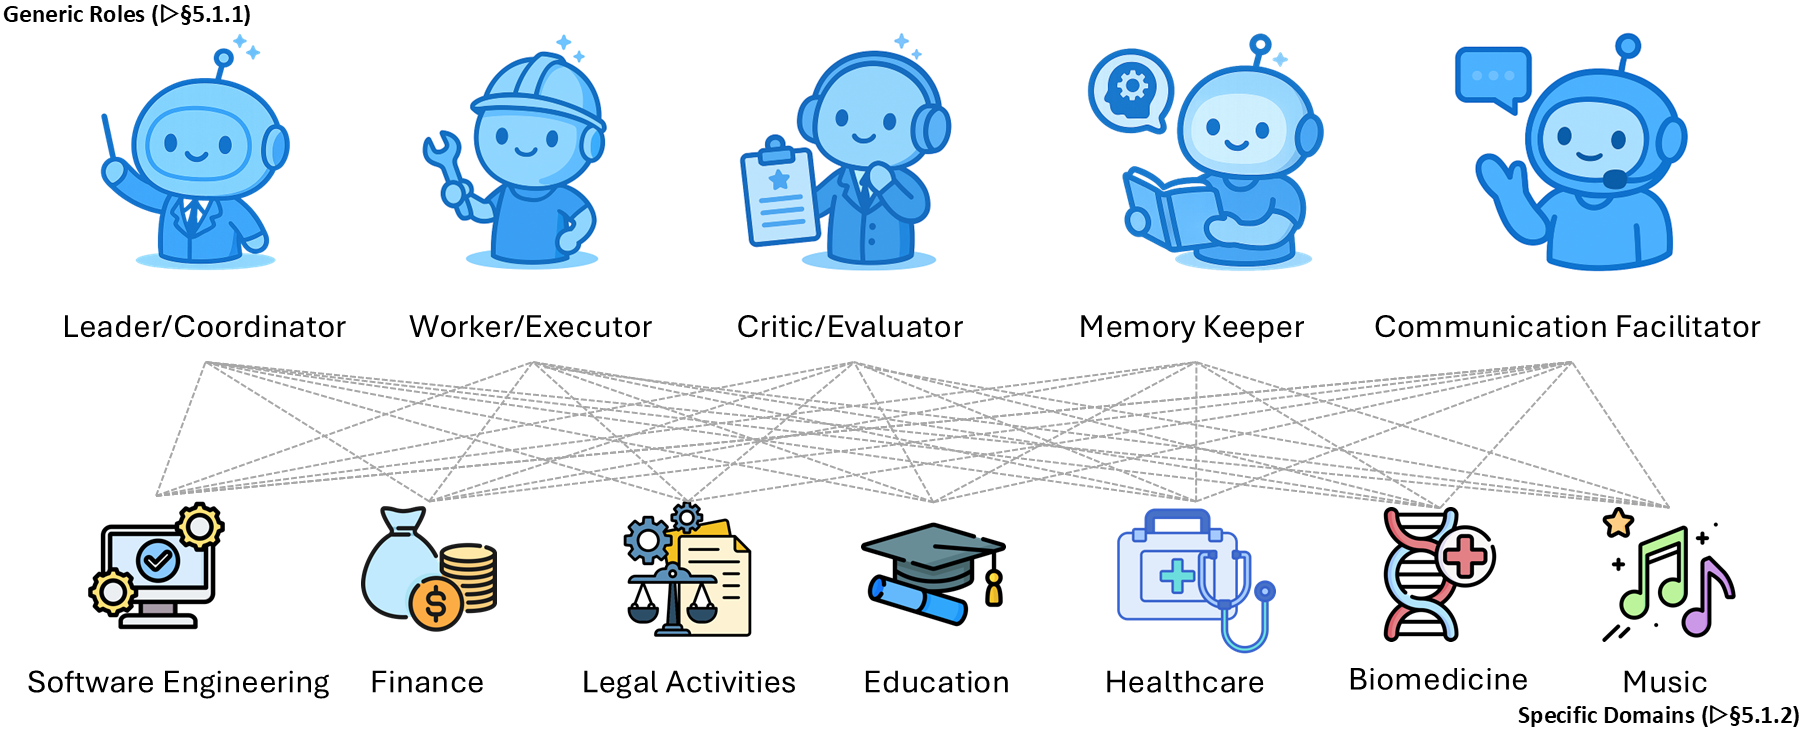
\includegraphics[width=0.8\linewidth]{arxiv/figs/mas.png}
    \caption{An overview of generic roles of agent and their specific domain adaptations in Section 5.1.}
    \label{fig:agentic_role}
\end{figure}

\subsubsection{Generic Roles}
\begin{itemize}[leftmargin=1.2em]
\item \textbf{Leader/Coordinator}: 
The leader, or coordinator, is responsible for maintaining high-level coherence within the system. 
This role involves setting global objectives, decomposing tasks into manageable subgoals, and assigning them to appropriate agents.
In addition, the leader arbitrates conflicts that emerge between agents with overlapping or contradictory outputs. 
In practice, this role often manifests itself as a meta-controller that monitors the progress of other agents and ensures that execution adheres to an overarching plan.
% sets goals, decomposes tasks, assigns roles, arbitrates conflicts.
\item \textbf{Worker/Executor}: 
Executors, often called workers, are the operational backbone of MAS. They engage in concrete actions such as invoking external tools, writing or executing code, retrieving documents, or interfacing with the environment. 
Although they typically act under the directives of a leader, well-designed systems allow for adaptive autonomy, 
where executors can refine or optimize their assigned tasks when new local information becomes available.
% performs tool calls, coding, retrieval, environment interaction.
\item \textbf{Critic/Evaluator}: 
The critic/evaluator role centers on quality assurance. This role includes verifying correctness, testing hypotheses, red-teaming responses, and surfacing potential risks. In LLM-based systems, this often corresponds to \emph{LLM-as-a-judge} setups, where dedicated evaluators assess the factuality, safety, or stylistic alignment of output. Critic roles help introduce checks and balances into otherwise generative workflows, thereby mitigating error propagation.
% verifies, tests, judges, or red-teams outputs; can be an \emph{LLM-as-a-judge}.
\item \textbf{Memory Keeper}: 
Effective MAS requires persistent memory to accumulate context, prevent repetitive failures, and enable learning across episodes. 
The memory keeper curates and maintains long-term knowledge structures such as episodic logs, semantic embeddings, retrieval indices, or knowledge graphs. 
By abstracting memory management into a dedicated role, the system can better balance short-term reactivity with long-term continuity and adaptation.
% curates episodic/semantic memory, retrieval indices, knowledge graphs.
\item \textbf{Communication Facilitator}:
Communication overhead can easily undermine MAS efficiency. 
This role governs protocols for inter-agent exchange, including defining message schemas, managing communication bandwidth, enforcing gating mechanisms, and orchestrating consensus-building. 
By reducing ambiguity and ensuring structured information flow, the communication facilitator prevents bottlenecks and coordination failures in large-scale or heterogeneous agent populations.
\end{itemize}


\subsubsection{Domain-Specific Roles}
Beyond generic agent roles, domain-specific tasks often require specialized functions. 
These roles reflect professional practices in particular industries and map naturally onto MAS architectures.

\textbf{Software Engineering}: 
In software engineering, MAS generally maps onto roles that mirror the software development lifecycle: \underline{\emph{architects}}, \underline{\emph{developers}}, \underline{\emph{code reviewers/testers}}, \underline{\emph{CI orchestrators}}, and \underline{\emph{release managers}}~\cite{hong2024metagpt,ChatDev}. 
The rationale is to distribute the responsibilities in a way that balances creativity, verification, automation, and governance, just as in industrial software practice.
\begin{itemize}
    \item Architects define system-level design principles and establish structural blueprints. 
    \item Developers translate these abstractions into concrete implementations. 
    \item Code reviewers and testers safeguard reliability, checking correctness, maintainability, and functional coverage. 
    \item CI orchestrators automate builds, testing, and artifact pipelines, reducing integration frictions. 
    \item Finally, release managers oversee deployment, aligning new versions with milestones and safety protocols.
\end{itemize}

Previous work has demonstrated similar mappings, such as MetaGPT~\cite{hong2024metagpt}, which decomposes development into Product Manager, Architect, and Engineer agents. ChatDev~\cite{ChatDev} further emphasizes communicative collaboration among specialized agents to support requirement analysis, coding, and testing. More recently, self-evolving collaboration networks have expanded this paradigm by enabling MAS to dynamically reorganize and optimize their roles throughout the software lifecycle~\cite{hu2024self}. A variant of MAS is also applied to the High-Performance Computing (HPC) domain~\cite{pauloski2025empowering}
By structuring MAS around these stages, the architecture gains the same robustness and scalability as professional engineering workflows.

\noindent \textbf{Finance}: 
The financial domain can be roughly decomposed into four archetypal roles: \underline{\emph{analysts}}, \underline{\emph{risk managers}}, \underline{\emph{traders/execution agents}}, and \underline{\emph{compliance officers}}~\cite{Chen2012, Hull2018}. This division reflects the established institutional design of financial organizations, where the responsibilities are segmented to balance profit generation with systemic stability.
\begin{itemize}
    \item Analysts operate at different levels (e.g., fundamental, sentiment, or technical), each extracting distinct signals from raw market or textual data.
    \item Risk Managers then monitor portfolio exposure, apply stress tests, and enforce safeguards to prevent cascading vulnerabilities. 
    \item Traders take responsibility for market interaction, while Execution agents ensure that orders are placed with speed and efficiency under liquidity constraints.
    \item Finally, Compliance roles ensure that activities remain aligned with regulatory requirements, enabling traceable decision-making and proper oversight.
\end{itemize}
Together, this layered ecology mirrors real-world financial institutions, where specialization and checks-and-balances are indispensable.
Recent advances in MAS for finance mirror this layered ecology. R\&D-Agent-Quant~\cite{R&D-Agent-Quant} demonstrates how agents can specialize in factor discovery and joint optimization for quantitative strategies. FinRobot~\cite{yang2024finrobot} provides an open source multi-agent platform tailored to financial applications, reflecting the practical need for modularity and scalability. PEER~\cite{wang2024peer} introduces expertization and tuning methods to adapt MAS to domain-specific responsibilities, while FinCon~\cite{finconf} highlights the role of conceptual verbal reinforcement to enhance decision-making and compliance. Together, these works underscore how MAS can replicate the specialization, checks, and balances of real-world financial institutions.


\textbf{Legal Activities}:
Multi-agent systems are also designed to model the collaborative and adversarial processes inherent in legal practice, with roles assigned to manage consultation, reasoning, and argumentation.
\begin{itemize}
    \item For legal consultation, frameworks often simulate a law firm's structure with a \underline{\emph{receptionist agent}} for client intake, specialized \underline{\emph{lawyer agents}} for providing advice, a \underline{\emph{secretary agent}} for documentation, and a \underline{\emph{boss agent}} for quality control. In a consultation model, the \emph{receptionist agent} first clarifies a user's query before routing it to the appropriate \emph{lawyer agent}. After the multi-turn consultation, the \emph{secretary agent} summarizes the interaction, and the \emph{boss agent} provides an evaluation, ensuring a comprehensive and high-quality service~\cite{sun2024lawluo}.
    \item For statutory reasoning, tasks are decomposed between \underline{\emph{knowledge acquisition agents}} that interpret legal texts and \underline{\emph{knowledge application agents}} that apply formalized rules to case facts. To be specific, in reasoning systems, the \emph{knowledge acquisition agent} first builds a reusable ontology from legal statutes; then, the \emph{knowledge application agent} uses this formal structure to analyze the specifics of a new case, ensuring consistent and transparent logic~\cite{sadowski2025verifiable}.
    \item To simulate courtroom dynamics, roles such as \underline{\emph{judge}}, \underline{\emph{plaintiff}}, \underline{\emph{defendant}}, and adversarial \underline{\emph{lawyer agents}} are created~\cite{chen2024agentcourt}. In courtroom simulations, adversarial \emph{lawyer agents} engage in debate before a \emph{judge agent}, reflecting on their performance after each trial to iteratively improve their argumentation strategies by updating their internal knowledge bases~\cite{chen2024agentcourt}.
\end{itemize}

\textbf{Education}:
In education, MAS is being developed to provide personalized and adaptive learning experiences by distributing pedagogical functions among specialized agents.
\begin{itemize}
    \item For personalized tutoring, a central \underline{\emph{tutor agent}} might engage a student using Socratic dialogue, while a \underline{\emph{memory dispatcher}} agent tracks the student's progress and misconceptions to adapt the difficulty and focus of the lesson in real-time~\cite{chudziak2025ai}.
    \item For curriculum design, a pipeline of agents collaborates: a \underline{\emph{research agent}} gathers relevant information, a \underline{\emph{planning agent}} structures it into a coherent course, and other agents generate specific learning activities or assessments. Also, it can be modeled by an adversarial process, where \underline{\emph{evaluator agent}} critiques a lesson plan created by \underline{\emph{generator agent}}, and \underline{\emph{optimizer agent}} refines it based on feedback~\cite{zhang2025eduplanner}. 
\end{itemize}

These systems demonstrate a shift towards creating intelligent, adaptive platforms that can support educators and provide students with more effective, engaging, and individualized learning journeys.

\textbf{Healthcare}:
In the healthcare domain, multi-agent systems are structured to mirror clinical and research workflows, distributing complex tasks among specialized AI agents.

\begin{itemize}
    \item For clinical diagnostics and consultation, these roles often include a \underline{\emph{triage agent}} (or \emph{moderator}) for initial case assessment, various \underline{\emph{specialist agents}} (e.g., pathologists, neurologists), a \underline{\emph{doctor agent}} for patient interaction, and a \underline{\emph{measurement agent}} to provide test results~\cite{kim2024mdagents, ghezloo2025pathfinder}. To be more specific, in the diagnostic setting, a \emph{triage agent} first assesses the complexity of a case and routes it to the appropriate \emph{specialist agents} for analysis. These specialists may then engage in multiround discussions, with a \emph{lead physician} agent synthesizing their opinions to reach a consensus. In addition to that, a \emph{doctor agent} conducts a multi-turn dialogue with a \emph{patient agent}, requesting specific data from a \emph{measurement agent} to gather information dynamically.
    \item For autonomous research, roles are modeled after the scientific process, featuring a \underline{\emph{meta agent}} for strategic planning, an \underline{\emph{executor}} for running analyses, an \underline{\emph{evaluator}} for assessing outcomes, and a \underline{\emph{reflector}} for synthesizing knowledge~\cite{zhu2025healthflow}. This division of labor allows for a systematic and comprehensive approach to multifaceted health challenges. Especially, the \emph{meta agent} plans an experiment, the \emph{executor} carries it out, the \emph{evaluator} provides immediate feedback, and the \emph{reflector} distills successful strategies into a persistent knowledge base, creating a self-improving cycle that enhances future planning.
    \item For public health events, ShortageSim~\cite{cui2025shortagesim} models FDA regulators, manufacturers, and healthcare buyers interacting under information asymmetry, enables counterfactual policy testing and evaluates how announcements and disruptions shape investment, stockpiling, and resolution timing against historical trajectories.
\end{itemize}

Other frameworks such as MMedAgent and MedAgent-Pro focus on orchestrating specialized medical tools, using a central agent to plan actions and aggregate results from various tool-based agents to handle multimodal data~\cite{li2024mmedagent, wang2025medagent}. 

\textbf{Biomedicine}:
In biomedicine, particularly in drug and material discovery, MAS is designed to automate and accelerate the scientific process by assigning roles that reflect the iterative cycle of design, testing, and refinement.

For de novo molecule design, key roles include the \underline{\emph{actor}} (or \emph{reasoner}) for generating novel structures, the \underline{\emph{evaluator}} for assessing chemical properties, and the \underline{\emph{self-reflector}} for refining future hypotheses based on results.
To be specific, the \emph{actor} agent proposes new candidates, which are then passed to the \emph{evaluator} agent. The evaluator uses computational chemistry tools to calculate properties like binding affinity and synthetic accessibility, providing quantitative feedback~\cite{averly2025liddia}. This feedback is then analyzed by the \emph{self-reflector} agent to update the system's strategy for the next generation cycle, creating a feedback-driven process of optimization~\cite{OSDA}.

Similarly, LIDDIA acts as a "digital chemist" with a \emph{Reasoner}, \emph{Executor}, \emph{Evaluator}, and \emph{Memory} component to navigate the drug discovery process and balance the exploration of new chemical spaces with the exploitation of promising candidates~\cite{averly2025liddia}. To streamline the creation of machine learning workflows, DrugAgent uses an \emph{LLM Planner} and an \emph{LLM Instructor} to automate programming for tasks like ADMET prediction~\cite{liu2024drugagent}. In genomics, GenoMAS orchestrates six specialized agents through a guided-planning framework to analyze complex gene expression data, integrating the reliability of structured workflows with the adaptability of autonomous agents~\cite{liu2025genomas}.

\textbf{Music}: In the creative domain of music composition, MAS is being explored to decompose the intricate process of creating music into collaborative, specialized roles. A system like ComposerX might feature a \underline{\emph{conductor agent}} that interprets a high-level user prompt and oversees the project, a \underline{\emph{melody agent}} that generates primary musical themes, a \underline{\emph{harmony agent}} that creates supporting chord progressions, and a \underline{\emph{rhythm agent}} that lays down the percussive and temporal foundation. These agents would interact iteratively, with the conductor agent synthesizing their outputs and providing feedback to ensure the different musical layers are coherent and aligned with the initial creative vision. This mirrors the collaborative process of a human orchestra or band, distributing creative responsibilities to achieve a complex and harmonious final product~\cite{ComposerX}.

\subsection{Collaboration and Division of Labor}

\begin{figure}
    \centering
    \resizebox{\linewidth}{!}{
    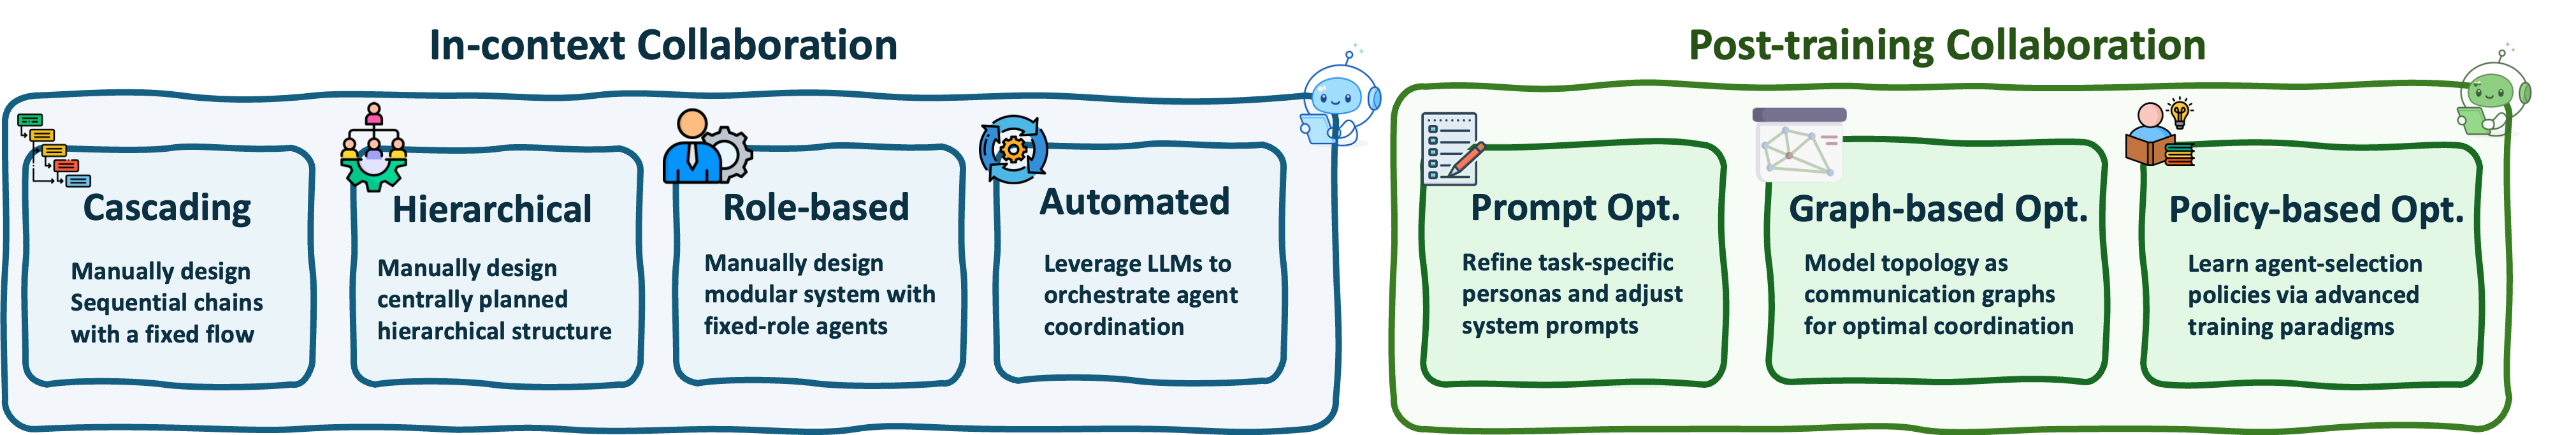
\includegraphics[width=\linewidth]{arxiv/figs/multi-agent-collab.png}
    }
    \caption{An overview of \textbf{Agentic Collaboration} in the multi-agent system, containing two parallel dimensions: in-context collaboration (training-free task-specific coordination design) and post-training collaboration (optimization-based automated workflow generation). }
    \label{fig:/multi_agent_collab}
\end{figure}

Collaboration and division of labor constitute a central organizing principle in modern multi-agent systems. Instead of treating agents as homogeneous components, recent work emphasizes how responsibilities are decomposed and coordinated across specialized agents to improve efficiency and robustness. From this perspective, existing approaches can be broadly organized along two dimensions. \textbf{In-context collaboration} focuses on coordination strategies that are specified or induced at inference time without additional training. \textbf{Post-training collaboration} instead optimizes agent roles, interaction structures, or routing policies through learning or search. In addition, \textbf{agentic routing} can be viewed as a special case of this division of labor, where routing decisions explicitly offload cognition and computation to different agents based on task demands.

\subsubsection{In-context Collaboration}
In the design of multi-agent systems, several studies have observed that leveraging task-specific in-context information is often sufficient to build highly effective systems without the need for explicit training. Among these works, one line of research relies on manually crafted pipelines, where researchers design the agent interactions and workflows tailored to the target task. In contrast, another line explores LLM-driven automatic pipeline generation, allowing the model itself to construct and adapt the system’s structure dynamically based on the task context.

\paragraph{Manually Crafted Pipelines.} 

These approaches rely on predefined hierarchies or fixed collaboration workflows, where agent roles, execution order, and communication rules are determined before execution. Hierarchical systems such as AgentOrchestra \cite{agentorchestra}, MetaGPT \cite{hong2024metagpt}, and SurgRAW \cite{low2025surgraw} feature a central planner or conductor directing subordinate agents through structured subgoals. Cascading pipelines like Collab-RAG \cite{xu2025collab}, MA-RAG \cite{marag}, Chain of Agents \cite{zhang2024chain}, and AutoAgents \cite{chen2023autoagents} process information sequentially, passing intermediate outputs downstream with limited revision. Modular role-decomposed frameworks such as RAG-KG-IL \cite{ragkgil}, SMoA \cite{smoa}, and MDocAgent \cite{han2025mdocagentmultimodalmultiagentframework} define fixed functional roles (e.g., retriever, reasoner, or vision agent) but allow minimal dynamic coordination. While these manually designed pipelines offer interpretability, modularity, and low execution complexity, their rigidity restricts adaptability to ambiguous or evolving reasoning tasks, motivating more flexible, reasoning-driven coordination mechanisms.





\paragraph{LLM-Driven Pipelines.}

This category leverages LLMs as orchestrators that decompose high-level goals into subgoals, route them to role-specialized agents or tools, and iteratively refine workflows based on intermediate feedback until completion. AutoML-Agent \cite{trirat2024automl} proposes a full-pipeline, orchestrator-led agent team that plans, assigns, and coordinates web/API/code tools through role-specialized micro-agents (e.g., coder/tester/runner), enabling end-to-end software development workflows. Magentic-One \cite{fourney2024magentic} introduces a generalist multi-agent system where a central Orchestrator plans, tracks progress, and performs ledger-based routing over specialized agents (WebSurfer, FileSurfer, Coder, ComputerTerminal), achieving competitive results on GAIA, AssistantBench, and WebArena. MAS-GPT \cite{ye2025mas} trains an LLM to emit executable MAS code conditioned on a user query, so a single forward pass generates a query-specific multi-agent workflow. MetaAgent \cite{zhang2025metaagent} presents a finite-state-machine (FSM) abstraction to declare states, transitions, and tools, from which a LLM designer automatically constructs the MAS pipeline. AOP \cite{li2024agent} formalizes orchestrator responsibilities and introduces three design principles, i.e., solvability, completeness, non-redundancy, and then operationalizes them with fast decomposition/assignment plus a reward-model evaluator.

\emph{Agent Routing.} Closely related to LLM-driven orchestration, a line of work explicitly models \textbf{agent routing} as a decision layer that selects appropriate specialists for each query or subtask. For example, AgentRouter \cite{zhang2025agentrouter} proposes a knowledge-graph-guided router that leverages structured task semantics to dispatch questions to relevant agents, enabling effective collaborative question answering without modifying individual agents. Similarly, Talk to Right Specialists \cite{wu2025talk} frames routing and planning as a unified inference-time process, where a controller dynamically assigns subtasks to domain-specialized agents based on intermediate reasoning states. These approaches highlight that agentic routing itself can be viewed as an inference-time realization of division of labor, where cognition is selectively offloaded to specialized agents.

\paragraph{Theory-of-Mind-Augmented Collaboration.}

Another interesting line of research is Theory of Mind (ToM), which refers to the ability of an agent to infer and reason about the beliefs, intentions, and mental states of other agents. \citet{li2023theory} first showed that equipping LLM agents with explicit belief-state representations in a cooperative text game improves both collaboration performance and the accuracy over ToM-free LLM baselines. Building on this, Hypothetical Minds~\cite{cross2024hypothetical} scaffolds ToM as a modular hypothesis-generation and refinement loop for other agents’ strategies, while MindForge~\cite{licua2024mindforge} extends ToM-aware reasoning to embodied collaborative learning. In parallel, \citet{wu2025large} provides a mechanistic account of how LLMs encode ToM, identifying sparse parameter patterns whose perturbation selectively disrupts social reasoning. Pushing toward, ToM-agent~\cite{yang2025large} augments LLM generative agents with counterfactual reflection over counterparts’ beliefs and BeliefNet~\cite{sagara2025beliefnest} offers a ToM-centric joint-action simulator where embodied agents act based on nested belief states. 




\subsubsection{Post-training Collaboration}

In multi-agent systems, the design of agent prompts (or personas) and the interaction topology plays a critical role in determining the system’s ability to solve complex tasks. Recently, optimizing these components during the post-training phase has emerged as an important research direction. Based on the optimization objective, existing studies can be broadly categorized into two lines of work: prompt optimization and topology optimization.

\textbf{Multi-agent Prompt Optimization.} Prompt optimization in multi-agent systems focuses on how agent roles, workflows, and feedback are encoded in prompts to yield reliable coordination and stronger task performance. For example, AutoAgents \cite{chen2023autoagents} extends prompt optimization from single-agent contexts to multi-agent teams, refining role specialization and execution plans through structured dialogue among meta-agents. SPP~\cite{unleashing2024} introduces a cognitive synergist that dynamically selects multiple personas during multi-agent collaboration for knowledge-intensive and reasoning-intensive tasks, enabling complementary expertise to emerge. DSPy Assertions \cite{singhvi2023dspy} introduces LM Assertions that can be either hard (Assert) or soft (Suggest). When violated, these assertions trigger backtracking and prompt revision using erroneous outputs and error traces. During compilation, the mechanism bootstraps examples and counterexamples to reinforce few-shot prompts, which improves both recall and accuracy. MASS \cite{zhou2025multi} demonstrates that prompts are often the dominant factor in MAS performance, and further applies automatic prompt optimization \cite{pryzant2023automatic} by incorporating local and global topology information to refine each agent’s prompt in a fine-grained manner.

As for topology optimization, two categories of research have emerged, each pursuing relatively independent optimization pathways. The first category of work treats the multi-agent topology as a communication graph, leveraging graph-based methods to identify an optimal structure that achieves strong performance under constrained communication costs (i.e., limited graph size). The second category adopts a policy-based perspective, where variable training paradigms are employed to learn an agent-selection policy with specially designed rewards or supervision signals. Through iterative, policy-based selection of subsequent agents, these approaches aim to progressively construct topologies that yield optimal overall performance. We discuss these two categories of approaches in greater detail in the following paragraphs.

\paragraph{Graph-based Topology Generation.} 
A large body of work models multi-agent systems (MAS) as graphs where agents are nodes, and inter-agent communication forms edges.  Then MAS design becomes a problem of learning the communication/coordination topology. These works could be roughly divided into three groups as follows. 

\emph{Graph generation.}
These methods aim to construct communication topologies from scratch by adaptively generating task-conditioned graphs. GommFormer \cite{hu2024learning} uses an encoder-decoder framework to learn the communication graph via continuous relaxation of the graph representation, optimizing topology end-to-end under bandwidth constraints. G-designer \cite{zhang2024g} starts from a task-anchored network with a virtual task node, then uses a variational graph auto-encoder to decode a query-adaptive communication graph. MCGD \cite{zenggraph} builds a sparse coordination graph with continuous node and discrete edge attributes, and performs categorical diffusion on edges and anisotropic diffusion on actions to capture structure diversity.

\emph{Graph pruning.}
These works start from dense collaboration graphs and aim to prune them into compact, task-appropriate pipelines while preserving utility and lowering token and compute costs.  For example, AgentPrune \cite{zhang2024cut} first formulates the MAS problem as a spatial-temporal graph sparsification problem, and then applies one-shot magnitude pruning to learn a sparse and effective pipeline. AGP \cite{li2025adaptive} learns a dual-pruning policy, i.e., soft-pruning on edges and hard-pruning on nodes, to acquire a per-query topology. G-Safeguard~\cite{wang2025g} introduces pruning as a security mechanism. It treats communication edges as the search space, employs a graph neural network to identify risky nodes, and applies deterministic rules to prune their outward edges based on a model-driven threshold, thereby defending the system against adversarial attacks. 

\emph{Topology search.}
This line of research explores the graph space by searching over agentic operators and communication edges to identify effective pipelines. Specifically, AFlow \cite{zhang2024aflow} automates multi-agent workflow design with Monte-Carlo Tree Search over a fixed library of operators. MASS pre-defines some influential graph motifs, such as debating and tool-using, and then implements topology search inside this pruned motif subset. Then MASS \cite{zhou2025multi} performs a prompt search on that topology to maximize performance. MaAS \cite{zhang2025multi} replaces single-graph search with a probabilistic “agentic supernet” over layered operator choices and uses a controller to sample a query-conditioned subgraph.  DynaSwarm \cite{leong2025dynaswarm} broadens the design space from a single optimized communication graph to a portfolio of candidate structures. It employs Actor–Critic (A2C) optimization to refine this portfolio and introduces a lightweight graph selector that chooses the most suitable topology for each instance. GPTSwarm \cite{zhuge2024gptswarm} formulates the search space as inter-agent connections within a computational graph. It relaxes the discrete topology into continuous edge probabilities and leverages reinforcement learning to optimize the resulting connection schemes, thereby enabling flexible and adaptive graph structures.

\paragraph{Policy-based Topology Generation.}

A growing line of research strengthens multi-agent pipeline generation by learning the policy of selecting subsequent agents with advanced training paradigms such as supervised fine-tuning (SFT), and reinforcement learning (RL). These approaches embed auxiliary signals into the optimization process, enabling agents to acquire stronger reasoning skills and more reliable coordination. Routing can be viewed as a special case of collaboration, in which a router conditions on task state and system context to learn a policy for selecting agents that maximize efficiency and performance \cite{yue2025masrouter,liu2025rcr,qian2025xrouter,wang2025optimal}. Broadly, these methods can be grouped into three categories based on the signal type they inject into learning.

\emph{Relative-advantage policy learning.}
Several approaches rely on critic-free objectives to form advantages, thereby avoiding centralized value models and providing effective guidance to optimize policy. For example,  MAGRPO \cite{liu2025llm} proposes a Dec-POMDP formulation for LLM collaboration and replaces centralized critics with a group-relative advantage signal, enabling decentralized training/execution at dialog-turn  granularity. MHGPO \cite{chen2025heterogeneous} extends GRPO-style signals to heterogeneous groups: it jointly optimizes different agent roles via a shared group-relative objective, and introduces practical sampling/optimization tweaks. COPY \cite{ma2024coevolving} utilizes two-agent co-training framework with shared rewards and KL regularization (to a frozen ref and cross-agent policies), improving stability and transfer between pioneer/observer roles on reasoning tasks.

\emph{LLM-generated prior guidance.}
Other methods leverage LLMs to generate rewards or priors for learning. Specifically, LGC-MARL \cite{jia2025enhancing} uses an LLM to propose a Reward Function Generator (RFG) that turns natural-language objectives into structured reward terms. LAMARL \cite{zhu2025lamarl} lets an LLM synthesize a prior policy and a task-specific reward function, then fine-tunes agents with RL. MAPoRL \cite{park2025maporl} defines rewards as weighted sums of LLM verifier scores on current and future turns, then updates policies with multi-agent PPO. COPPER \cite{bo2024reflective} learns a shared reflector with a counterfactual-PPO pipeline in which a learned reward model scores each agent’s reflection by its marginal contribution to task improvement. SIRIUS \cite{zhao2025sirius} builds an experience library by retaining trajectories that lead to successful outcomes and augmenting failures, while a Judgment–Critic–Actor triad supplies LLM-generated correctness signals that filter and supervise subsequent fine-tuning across reasoning tasks. Multiagent Finetuning \cite{subramaniam2025multiagent} bootstraps reasoning by running multi-agent debates among generator LLMs and using LLM critics plus majority voting to produce self-generated supervisory signals, then fine-tunes role-specialized agents on critic-selected trajectories to improve both accuracy and diversity.

\emph{Human preference signals.}
This line of research replaces or augments environment rewards with human-derived feedback to align behavior with human intent, in both online and offline regimes. For instance, M3HF \cite{wang2025m3hf} organizes human input into multi-phase feedback (e.g., scalar ratings, pairwise comparisons, and natural-language rationales) processed by LLMs into reward shaping signals. O-MAPL \cite{bui2025mapl} introduces an end-to-end preference-based learning framework and directly learns Q-values from offline preference data, bypassing the two-stage reward-model-then-RL pipeline. 


\subsection{Multi-Agent Evolution}

While self-evolving agents enable individual models to continuously improve through interaction and feedback, many real-world applications require collective intelligence supported by cooperation among multiple agents. Therefore, recent studies extend self-evolution from single-agent settings including planning, tool-use, and search evolution~\cite{shinn2023reflexion, sun2023adaplanner, madaan2023self, wang2025ragen, wang2023voyager} to multi-agent co-evolution, where adaptation emerges across distributed agents~\cite{zhang2024aflow, 10.1145/2970276.2970311, wan2025rema, feng2025group, ke2025mas}. Beyond evolving model parameters, memory, prompts, and tools~\cite{chhikara2025mem0, zhao2024expel, khattab2024dspy, qiu2025alita}, multi-agent evolution further targets shared memory, communication mechanisms, and collaboration protocols~\cite{zhou2025multi, ke2025mas, Wang2024AgentWM}. 

As a result, multi-agent memory must jointly evolve along architecture, topology, content, and management dimensions, supported by hierarchy-structured, role-aware architectures \cite{zhang2025gmemory}, governed and distributed storage topologies \cite{xu2025sedm, rezazadeh2025collaborative}, modular and task-structured memory contents \cite{wang2025mirix, han2025legomem}, and active management mechanisms for compression, verification, and continual updating \cite{kaiya2023lyfe, tang2025agent} to ensure coherent and scalable collaboration.

The goal thus shifts from optimizing a single agent’s capability to improving the collective performance of multiple agents on complex, long-horizon tasks~\cite{zhang2024aflow, 10.1145/2970276.2970311, wan2025rema,novikov2025alphaevolve}.

\subsubsection{From Single-Agent Evolution to Multi-Agent Evolution}


While the shift from single-agent evolution to multi-agent co-evolution broadens the spatial dimension of adaptation from an individual model to a collective, the temporal dimension of evolution remains equally crucial. Beyond determining who evolves (a single agent or a population), recent studies also investigate when and how fast agents should adapt during interaction. This perspective leads to a complementary axis of analysis that distinguishes short-horizon, within-episode updates from long-term, cross-episode improvements, commonly referred to as intra-test-time evolution and inter-test-time evolution. We summarize these temporal modes of self-evolving behavior.

Intra-test-time evolution refers to the ability of agents to adapt and improve during task execution, enabling them to correct failures and refine strategies on the fly when facing unseen states or unexpected feedback. Unlike static inference pipelines, this paradigm embeds self-reflection, dynamic planning, memory rewriting, or even localized fine-tuning into the execution loop. Representative works leverage natural-language self-critique~\cite{shinn2023reflexion, madaan2023self} and runtime adaptive planning~\cite{sun2023adaplanner, hua2024trustagent} to generate corrective signals without external supervision. Reflexion~\cite{shinn2023reflexion} allows agents to store distilled reflective feedback for immediate behavior improvement, while AdaPlanner~\cite{sun2023adaplanner} dynamically revises and replans mid-trajectory based on environmental mismatch detection. Beyond contextual adaptation, methods such as test-time supervised updating~\cite{zweiger2025self} and test-time reinforcement learning (TTRL)~\cite{zuo2025ttrl, simonds2025ladder} directly modify model behavior when encountering difficult cases, often through problem-variant generation and targeted optimization. These approaches demonstrate that performance at inference time can improve within a single episode, forming short-horizon adaptation loops where the model learns while solving, rather than merely executing a fixed policy.


Inter-test-time evolution extends the self-improving process to across-task learning, where adaptations made in one task can be consolidated and transferred to future tasks. This enables the accumulation of persistent, generalizable capabilities over a lifelong interaction stream. A prominent paradigm involves offline self-distillation, where the agent generates responses and then refines them via self-evaluation before using them for supervised fine-tuning-such as in SELF~\cite{lu2023self}, STaR~\cite{zelikman2022star}, and Quiet-STaR~\cite{ferrag2025reasoning}. These methods turn incorrect initial reasoning into high-quality labeled data for future performance gains. Additionally, online reinforcement learning frameworks such as RAGEN~\cite{wang2025ragen} and DYSTIL~\cite{wang2025dystil}  continuously update policies based on dense interaction feedback, allowing agents to gradually internalize complex decision-making strategies over long horizons. Inter-test-time evolution can also incorporate curriculum mechanisms that automatically adjust task difficulty and environment complexity~\cite{qi2024webrl, lee2024animals}, as well as experience structuring via memory evolution to preserve accumulated reasoning heuristics~\cite{liang2025sage, salama2025meminsight, Wang2024AgentWM}. This temporal mode focuses on stable long-term improvement, transforming short-lived corrections from individual tasks into continual competence growth across diverse task distributions.

To support these new capabilities, mechanisms evolve from individual reward-based or reflective adaptation~\cite{lu2023self, kumar2024training, yuksekgonul2024textgrad} to multi-agent reinforcement learning and game-theoretic co-optimization~\cite{wan2025rema, feng2025group}, enabling collaborative structures to self-organize under evolving task requirements. Moreover, memory-driven multi-agent evolution (e.g., shared workflow memory or knowledge graphs) helps maintain accumulative group intelligence across episodes~\cite{Wang2024AgentWM, li2025memos}.
Overall, multi-agent evolution transforms isolated self-improvement loops into adaptive intelligent ecosystems capable of self-correction, self-organization, and social learning. This transition marks a critical step toward artificial collective intelligence, where cooperative dynamics drive continuous progress beyond the capabilities of any individual agent~\cite{zhou2025multi, zhang2024aflow, 10.1145/2970276.2970311, latentmas}.


\begin{figure}
    \centering
    \resizebox{0.6\linewidth}{!}{
    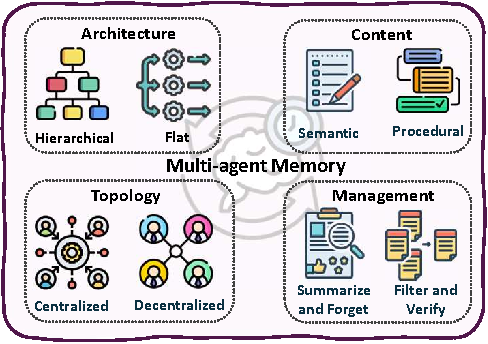
\includegraphics[width=\linewidth]{arxiv/figs/multi-agent-memory.pdf}
    }
    \caption{\textbf{Four dimensions of multi-agent memory design.} 
    The framework includes (1) \textbf{Architecture}, how memory is structured; 
    (2) \textbf{Topology}, where it is stored and shared; 
    (3) \textbf{Content}, what type of knowledge is stored; and 
    (4) \textbf{Management}, how it is maintained and updated.}
    \label{fig:multi_agent_memory}
\end{figure}

\subsubsection{Multi-agent Memory Management for Evolution}


Multi-agent LLM systems pose unique challenges for memory design compared with single-agent settings. 
Beyond maintaining an individual agent's local context, they must capture inter-agent interactions, track roles and dependencies over time, and preserve both shared and private knowledge coherently. 
Memory must also remain scalable as collaboration grows and interactions accumulate. 
To provide a clearer understanding of this landscape, \textbf{we categorize existing approaches along four key dimensions}: 
(1) \textit{architecture}, how memory is organized within and across agents; 
(2) \textit{topology}, whether it is centralized, distributed, or hybrid; 
(3) \textit{content}, the type and structure of stored knowledge; and 
(4) \textit{management}, how memory is written, retrieved, and updated over time. Illustrations are shown in Figure \ref{fig:multi_agent_memory}.

% ============================================================
% DIMENSION 1: ARCHITECTURE
% ============================================================

\paragraph{Architecture Dimension: Hierarchical and Heterogeneous Designs.}

Recent work highlighted that prevailing multi-agent memory mechanisms were overly simplistic and lacked per-agent customization~\cite{zhang2025gmemory}. To address this, G-Memory constructs a three-tier graph hierarchy (insight, query, interaction graphs) that separates high-level generalizable insights from fine-grained execution traces. This hierarchical approach enables bi-directional memory traversal for retrieving both abstract lessons and concrete precedents across episodes. However, instead of global aggregation, Intrinsic Memory Agents adopts an opposing strategy by maintaining dedicated role-aligned memory templates for each agent~\cite{yuen2025intrinsic}. This heterogeneous approach preserves specialized perspectives on collaborative planning benchmarks by reducing irrelevant information per agent. Recent work further explores hybrid strategies, with some systems employing adaptive hierarchical knowledge graphs in decentralized architectures that allow agents to reason over past interactions and share only relevant information rather than raw experiences~\cite{yang2025damcs}. These contrasting approaches reveal a fundamental trade-off: hierarchical designs optimize for global coherence and cross-episode learning, while heterogeneous designs optimize for role fidelity and computational efficiency.

% ============================================================
% DIMENSION 2: TOPOLOGY & GOVERNANCE
% ============================================================

\paragraph{Storage Topology and Memory Governance.}

Systems employ different topologies to balance scalability, privacy, and coherence, each reflecting different assumptions about trust and coordination. SEDM (Self-Evolving Distributed Memory)~\cite{xu2025sedm} tackles memory management by turning memory into an active, self-optimizing component through verifiable write admission (via reproducible replay) and utility-based consolidation. This centralized approach with verification gates ensures that only factual or useful information enters the repository and performs cross-domain knowledge diffusion to enable transfer across heterogeneous tasks. In contrast, when privacy and organizational boundaries matter, Collaborative Memory ~\cite{rezazadeh2025collaborative} distinguishes private versus shared memory fragments using bipartite graph policies. Every entry carries immutable provenance (source agent, accessed resources, timestamp), enabling compliance auditing and safe cross-agent knowledge transfer in federated systems. At the other end of the spectrum, some systems like Memory Sharing~\cite{gao2024memory} adopt uncontrolled pooling where all agents freely exchange experiences in a shared memory pool. Research shows that memory sharing among LLM agents leads to a more diverse collective memory pool, which improved performance on open-ended tasks by creating emergent collective intelligence. These three topologies represent increasing levels of formality and control, reflecting different priorities for managing the trade-off between knowledge diversity and verification rigor.

% ============================================================
% DIMENSION 3: GRANULARITY
% ============================================================

\paragraph{Memory Content: Semantic, Task, and Cognitive-Phase Decomposition.}

Different content decomposition strategies suit different task characteristics, and the choice of content structure fundamentally shapes how agents interact with memory. 
MIRIX~\cite{wang2025mirix} pioneered \textit{semantic decomposition} by defining six specialized memory types (Core, Episodic, Semantic, Procedural, Resource, Knowledge Vault) managed by distinct agents, achieving a 35\% accuracy gain on multimodal QA tasks while reducing storage through flexible routing. 
Building on this modular principle, LEGOMem~\cite{han2025legomem} instead employs \textit{task-based decomposition}, breaking execution traces into reusable memory units flexibly assigned to either central planners or specialist task agents. 
This design shows that orchestrator memory improves task decomposition and delegation, while agent memory enhances subtask execution, effectively narrowing performance gaps between small and large LLM teams. 
Recently, MAPLE introduced Cognitive-phase Decomposition~\cite{bai2025maple}, using specialized agents (Solver, Checker, Reflector, Archiver) to enable systematic error detection and plan repair cycles. 
The Reflector diagnoses errors after each episode, and the Archiver stores refined plans to avoid repeated mistakes, supporting feedback-driven learning. 
These three content decomposition strategies reveal that memory design should align with task structure: semantic content for heterogeneous information, task-based for workflow automation, and cognitive-phase for error-sensitive reasoning.

% ============================================================
% DIMENSION 4: MANAGEMENT
% ============================================================

\paragraph{Memory Management Strategies.}

Effective long-term memory requires active management balancing relevance, efficiency, and coherence through different approaches that trade off simplicity against sophistication. Lyfe Agents~\cite{kaiya2023lyfe} pioneered the forgetting-based approach using Summarize-and-Forget mechanisms to regularly compress memory, retaining only critical context. This strategy is suitable when storage is severely constrained, though it risks losing nuanced details for edge cases. To improve upon simple forgetting, AGENT-KB~\cite{tang2025agent} introduced more sophisticated management by organizing procedural traces into structured (entity, action, observation) triples and learning pattern abstractions reusable across tasks. Agents collaborate to retrieve, update, and reason over memory segments, enabling generalization without explicit retraining while central coordination ensures long-term consistency for scalable embodied planning. The choice among these strategies depends on system priorities: forgetting prioritizes storage efficiency, verification prioritizes reliability, and learning-based approaches prioritize adaptability. Production systems typically combine strategies, e.g., verification for critical memories and forgetting for low-utility peripheral information, to balance multiple objectives.

% ============================================================
% FUTURE DIRECTIONS
% ============================================================

\paragraph{Discussions.}

Despite substantial progress, multi-agent memory systems remain largely unexplored with respect to post-training and model adaptation. Current approaches focus primarily on memory organization and retrieval for pre-trained models, with little investigation into how multiple agents can jointly optimize their memories through post-training procedures such as reinforcement learning or supervised fine-tuning. This represents a notable gap: while post-training techniques have been actively explored for single-agent memory systems, extending them to enable multi-agent teams to co-evolve their memory structures and management policies remains an open problem.




\subsubsection{Training Multi-agent to Evolve}

Recent advancements have shifted multi-agent systems from fixed, hand-designed coordination toward training paradigms that enable agents to evolve over time \cite{ma2024coevolving, multi-agent-evolve, zhao2025sirius}. Training multi-agent systems to evolve represents a critical step toward realizing adaptive, long-horizon intelligence beyond static coordination. In this emerging paradigm, agents improve collectively through interaction, feedback, and shared memory, rather than isolated or independently optimized behaviors. By embedding reasoning into the learning loop, via reinforcement learning \cite{marft}, self-play \cite{strongermas}, curriculum evolution \cite{park2025maporl}, and verifier-driven feedback \cite{marlhf}, multi-agent systems can internalize coordination strategies, address inter-agent credit assignment, and progressively refine divisions of labor. This evolution transforms multi-agent reasoning from a static ensemble of cooperating LLMs into a self-improving organization that adapts its structure, communication patterns, and policies in response to task complexity and environmental change \cite{zhao2023chatenvironmentinteractivemultimodal}.

\paragraph{Co-evolution via Interaction and Intrinsic Feedback.}
A growing body of work has operationalized multi-agent evolution through explicit training objectives that couple interaction, feedback, and role specialization. For instance, Multi-Agent Evolve \cite{multi-agent-evolve} instantiates a closed-loop co-evolution framework containing three interacting roles (\emph{Proposer}, \emph{Solver}, and \emph{Judge}), all of which are derived from a shared LLM backbone and jointly optimized via reinforcement learning. This forms a self-improving curriculum that enables collective skill growth without external supervision. In a related spirit, CoMAS \cite{CoMAS} emphasizes intrinsic interaction rewards, extracting learning signals directly from multi-agent discussion dynamics through an LLM-based judge, thereby enabling decentralized co-evolution driven purely by collaborative interaction.

\paragraph{Multi-Agent Reinforcement Fine-Tuning for Collective Adaptation.}
Additional works have focused on principled reinforcement fine-tuning frameworks tailored to LLM-absed multi-agent systems. For example, MARFT \cite{marft} formalizes multi-agent reinforcement fine-tuning by highlighting key mismatches between classical MARL assumptions and LLM-based agent organizations, such as role heterogeneity, dynamic coordination, and long-horizon dialogue, and provides a systematic framework for stabilizing collective post-training. Stronger-MAS \cite{strongermas} further adapts on-policy reinforcement learning to multi-role, multi-turn settings by introducing agent- and turn-wise grouping strategies that extend GRPO-style optimization, enabling more effective coordination learning across complex agent workflows. Similarly, MAPoRL \cite{park2025maporl} proposes multi-agent post-co-training, where multiple LLMs are jointly optimized using a collaboration-aware verifier that rewards not only final outcomes but also the quality of intermediate discussions, encouraging the emergence of transferable communication strategies.

\begin{figure}[!t]
    \centering
    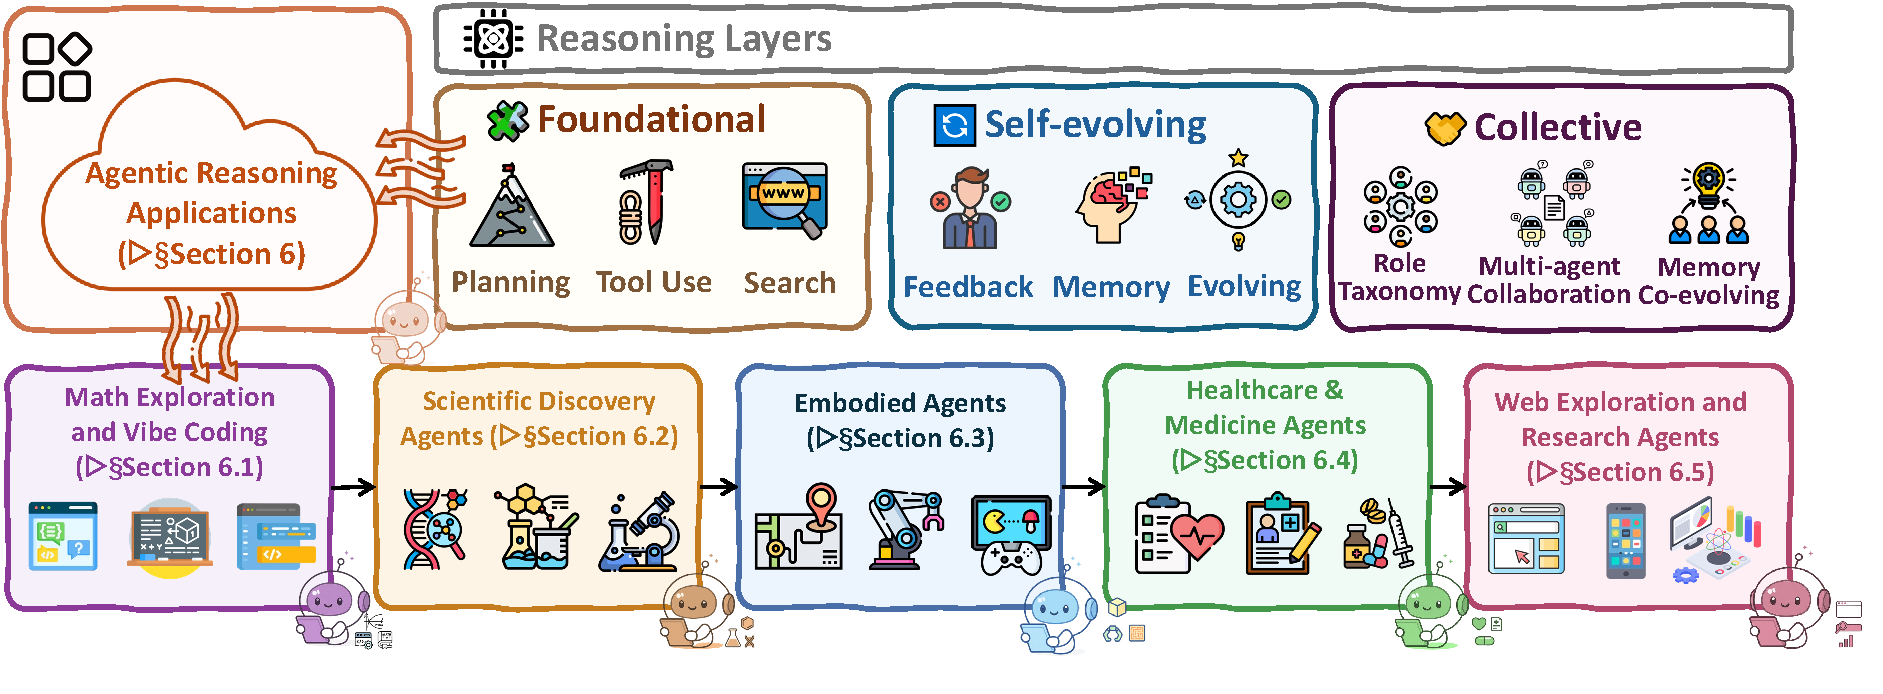
\includegraphics[width=\linewidth]{arxiv/figs/application.pdf}
    \caption{An overview of the applications of agentic reasoning.}
    \label{fig:application}
\end{figure}

\paragraph{Role Specialization and Joint Credit Assignment.}
Other approaches have explored structured role specialization and joint credit assignment. MALT \cite{MALT} trains sequential pipelines of heterogeneous agents using trajectory expansion and outcome-based reinforcement signals, allowing each agent to improve its specialized function while optimizing end-to-end collaborative performance. MARS \cite{mars} extends this idea to long-horizon research settings by jointly training complementary System~1 (fast, intuitive) and System~2 (deliberate, tool-using) agents via multi-agent reinforcement learning, enabling adaptive division of labor under complex tool interactions.

\paragraph{Preference- and Alignment-Driven Multi-Agent Evolution.}
Finally, another line of work has studied evolution under preference- and alignment-driven objectives. Preference-based multi-agent reinforcement learning \cite{marlhf} studies how collective policies and equilibria can be learned from preference-only feedback, addressing data coverage and stability challenges inherent in multi-agent settings. From a safety perspective, Alignment Waltz \cite{alignment-waltz} frames alignment as a cooperative co-evolution process between a generation agent and a feedback agent, where evolving guidance enables the system to iteratively refine unsafe or unhelpful behaviors. Collectively, these methods demonstrate how embedding reinforcement learning, co-evolution, and verifier-driven feedback into multi-agent training enables LLM-based systems to evolve from static collaborations into adaptive, self-improving organizations.